% Para facilitar a manutenção é sempre melhore criar um arquivo por capitulo, para exemplo isso não é necessário 

%---------------------------------------------------------------------------------------
\chapter{Descrição da execução do experimento}
Utilizou-se o Quartus, na versão 13 SP1, para a criação virtual do circuito, uma FPGA Cyclone II - EP2C20F484C7.
Analisando o problema proposta, chegou-se na expressão lógica
$$ P + G + \simV$$
com P representando \textit{porta aberta}, G \textit{gelo} e V \textit{vazamento de gás}

\begin{figure}[htb]
    \centering
	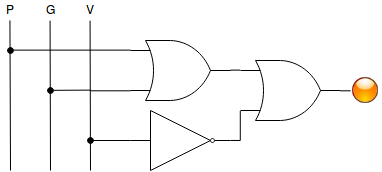
\includegraphics{img/desenhoCircuito}
	\caption{\label{fig_logo}Desenho do circuito}
	\legend{Imagem do circuito feito no Quartus}
\end{figure}

\begin{tabular}{c|c|c|c}
%\hline
\textbf{P} & \textbf{G} & \textbf{V} & \textbf{P+G+($\sim$V)} \\
\hline
0 & 0 & 0 & 0\\\hline
0 & 0 & 1 & 1\\\hline
0 & 1 & 0 & 1\\\hline
0 & 1 & 1 & 1\\\hline
1 & 0 & 0 & 1\\\hline
1 & 0 & 1 & 1\\\hline
1 & 1 & 0 & 1\\\hline
1 & 1 & 1 & 1
\end{tabular}



Apresentar   o   detalhamento   da  execução  e   resultados   dos   passos   realizados 
durante   o   experimento,   incluindo   tabelas   verdade,   esquemáticos,   e   código 
(quando  houver). 
Especificar  componentes,  sistemas  e  instrumentos  utilizados. 
Usar listas, figuras e quadros, descrevê-los e discuti-los.



%---------------------------------------------------------------------------------------